\documentclass{llncs}
\usepackage[utf8x]{inputenc}
\usepackage[english, russian]{babel}
\usepackage{url}
\usepackage{amsmath, amssymb, amsfonts, amsbsy, bm}
\usepackage{mathtools}
\usepackage{graphicx}
\usepackage{stfloats}
\usepackage{caption}
\usepackage{pgf, tikz}
\usepackage{mathtools}
\usepackage{textcomp}
\usetikzlibrary{shapes,arrows}
\setcounter{totalnumber}{10}
\setcounter{topnumber}{10}
\usepackage{ dsfont }
\begin{document}


\title{Сравнение методов построения полярных кодов для каналов с аддитивным белым гауссовским шумом}


\author{Глеб Балицкий \inst{1,2}, Андрей Дзись \inst{1,2}, Алексей Фролов \inst{3,1} }
\institute{Институт Проблем Передачи Информации РАН, Москва, Россия, \and  Московский физико-технический институт, Москва, Россия \and Сколковский институт науки и технологий, Москва, Россия \\
\email{ gleb.balitskiy@phystech.edu,  andrey.dzis@phystech.edu, al.frolov@skoltech.ru}}




\maketitle          
%DONE
\begin{abstract} В работе рассматривается методы построения полярных кодов для каналов с аддитивным белым гауссовским шумом. Путем моделирования были исследованы два метода: метод эволюции плотности и метод построения кодов на основе верхней оценки параметров Бхаттачариa. В ходе исследования было произведено сравнение работы данных методов, были получены оптимальные параметры построения кода для разных отношений сигнал-шум (SNR). 
\\

\
%DONE
\textbf{Ключевые слова:} Построение  полярных кодов, каналы с аддитивным белым гауссовским шумом, декодирование методом последовательного исключения (successive cancelation).
\end{abstract}

\section{Введение}
Конструкция полярных кодов и оценки оптимальных параметров были предложены в [1], исследования были продолжены в [2]. Данные коды являются первыми известными кодами с субквадратичной сложностью кодирования и декодирования, для которых доказан факт достижения пропускной способности дискретных двоичных каналов без памяти, например, бинарного канала со стираниями (BEC). Вследствие особенностей построения кода, его структура непосредственно зависит от SNR в канале. Таким образом, актуальной задачей является нахождение таких параметров кода, при которых код может работать на некотором заранее заданном диапазоне SNR.
\\
Основные результаты работы заключаются в следующем. Основываясь на предыдущих работах,  была произведена симуляция работы кодера, декодера последовательного исключения  и передачи данных по двум моделям канала: двоично-симметричному с аддитивным белым гауссовским шумом. Для каналов с гауссовским шумом было произведено исследование  на заданном диапазоне SNR эффективности кода, дизайн которого соответствует определенному значению SNR. 



%Расширенное введение в работу. Тут необходимо написать про актуальность работы, что делалось до этого и что сделано в работе

\section{Предварительные сведения}
\subsection{Полярные коды}
Введем понятия двух наиболее важных величин для дискретных двоичных симметричных каналов без памяти(B-DMC):  симметричной пропускной способности
\begin{equation}
    I(W) \triangleq \sum\limits_{y\in\mathcal{Y}} \sum\limits_{x\in\mathcal{X}}\frac{1}{2}W(y|x)\log\frac{W(y|x)}{\frac{1}{2}W(y|0)+\frac{1}{2}W(y|1)}
\end{equation}
и параметра Бхаттачариa
\begin{equation}
    Z(W) \triangleq \sum\limits_{y\in\mathcal{Y}} \sqrt{W(y|0)W(y|1)}
\end{equation} Эти параметры используются как показатели скорости и надежности, соответственно.
\\
Принцип работы полярных кодов построен на явлении поляризации канала. Явление заключается в следующем: мы из набора $N$-независимых копий данного B-DMC канала можем создать второй набор $N$ двоичных каналов $W_N^{(i)}: 1\leq i\leq N$ так, что с увеличением $N$ для $i$, для которых $I(W_N^{(i)})$ стремится к 1, пропускная способность соответствующих каналов достигает $I(W)$.Соответственно, для $i$, для которых $I(W_N^{(i)})$ стремится к 0, достигает значения $1-I(W)$. Таким образом, для передачи достаточно выбирать из этих каналов лишь те,пропускная способность которых стремится к 1. Коды, построенные по данному принципу, называются полярными. 
Двоичный симметричный канал без памяти называется каналом со стиранием (BEC) , если для каждого $y\in\mathcal{Y}$ выполнено:
\begin{equation}
    W(y|0)W(y|1)=0 
\end{equation}
или 
\begin{equation}
    W(y|0)=W(y|1)
\end{equation}
В таком случае $y$ называется символом стирания. Соответственно, $W(y|0)$ называется вероятностью стирания.
\\

На примере BEC рассмотрим подробнее поляризацию канала, состоящую из двух этапов: объединение  и разделение канала.
В объединении основная задача рекурсивно получить вектор $W_N:\mathcal{X}^N \rightarrow \mathcal{Y}^N$. Рекурсия начинается с $n = 0$ (нулевой шаг рекурсии) с единственной копией канала $W$ и $W_1 \triangleq W$ Первый шаг $n = 1$ начинается с двух независимых копий $W_1$ и составляет $W_2: \mathcal{X}^2 \rightarrow \mathcal{Y}^2$ (см.рис.1) с вероятностью ошибки:
\begin{equation}
    W_2(y_1,y_2|u_1,u_2) = W(y_1|u_1 \oplus u_2)W(y_2|w_2)
\end{equation}
\\
\begin{figure}[!h]
\centering
\tikzset{%
  block/.style    = {draw, thick, rectangle, minimum height = 3em,
    minimum width = 3em},
  sum/.style      = {draw, circle, node distance = 2cm}, % Adder
  input/.style    = {coordinate}, % Input
  output/.style   = {coordinate} % Output
}
% Defining string as labels of certain blocks.
\newcommand{\suma}{\Large$+$}
\newcommand{\inte}{$\displaystyle \int$}

\begin{tikzpicture}[auto, thick, node distance=2cm, >=triangle 45]
\draw
% Drawing the blocks of first filter :
	node at (0,0)[right=-3mm]{\Large \textopenbullet}
	node [input, name=input1](input1){} 
	node at (0,-2)[right=-3mm]{\Large \textopenbullet}
	node[input,name=in2](in2){}
	node at (2,-2) {\textbullet} 
	node [sum, right of=input1] (suma1) {\suma}
	node [block, right of=suma1] (inte1) {\Large $W$}
	node [block, below of=inte1] (inte2) {\Large $W$}
	node at (6,0)[right=-3mm]{\Large \textopenbullet}
	node [input, name=output1](output1) {}
	node at (6,-2)[right=-3mm]{\Large \textopenbullet}
	node [input, name = output2](output2){}
	;
	\draw[->] (input1) -- node {$u_1$}(suma1);
	\draw[->](0,-2) -- node{$u_2$}(2,-2);
	\draw[->](2,-2) -- node{}(suma1);
	\draw[->](suma1) -- node{$x_1$}(inte1);
	\draw[->](2,-2) -- node{$x_2$}(inte2);	
	\draw[->](inte1) -- node{$y_1$}(5.889,0);
	\draw[->](inte2) -- node{$y_2$}(5.889,-2);
	
\end{tikzpicture}
\caption{}
\end{figure}
\\
%Общая форма рекурсии представлена на рисунке 2. Две независимые копии $W_{N/2}$ составляют $W_N$. 

В результате входной вектор $u_1^N$ преобразуется в вектор $s_1^N$ так, что $s_{2i-1} = u_{2i-1} \oplus u_{2i}$, $s_{2i}=u_{2i} $
\\
Разделение канала заключается в делении $W_N$ в последовательность $N$ бинарных каналов $W_(i)^N : \mathcal{X} \rightarrow \mathcal{Y}^N \times \ \mathcal{X}^{i-1}, 1\leq i \leq N$ с пропускными способностями:
\begin{equation}
    W_N^{(i)}(y_1^N,u_1^{i-1}|u_i) \triangleq \sum\limits_{u^N_{i+1} \in\mathcal{X}^{N-i}} \frac{1}{2^{N-1}}W_N(y_1^N|u_1^N)
\end{equation}
\\ 
Построение кода будем производить над двоичным полем $GF(2)$. Для двух векторов $a_1^N$ и $b_1^N$ через $a_1^N \oplus b_1^N$ обозначим покомпонентное суммирование по модулю 2. 
%Для матриц $A=[A_{ij}]$ размерности $m \times n$ и $B=[B_{ij}]$ размерности $r \times s$ произведение Кронекера определяется как:
%\begin{equation}
%    A\otimes B = \begin{bmatrix}
%A_{11}B & \cdots & A_{1n}B \\
%\vdots & \ddots & \vdots \\
%A_{m1}B & \cdots & A_{mn}B
%\end{bmatrix} 
%\end{equation}
%матрица размерности $mr \times ns$. 

Степень $A^{\otimes n}$ определяется как $A \otimes A^{\otimes (n-1)}$  для $n \geq 1$. Для $n = 0$ определим $A^{\otimes 0} \triangleq [1]$.
Пусть на вход кодера подается последовательность векторов $x^N_1$ длины $N = 2^n$, тогда, обозначая последовательность кодовых слов $u_1^N$, получаем равенство:
\begin{equation}
    x^N_1 = u_1^NG_N
\end{equation}
где $G_N$ порождающая матрица, равная:
\begin{equation}
    G_N = B_N F^{\otimes n}
\end{equation}
где $B_N$ матрица перестановки, а $F^{\otimes n} = F \otimes F^{\otimes (n-1)}$, где $F \triangleq  \begin{bmatrix}
1  & 0  \\
1  & 1 \\
\end{bmatrix} $
%Тут необходимо четко определить предмет исследования, дать определение полярных кодов, что такое  двоичный стирающий канал и как полярные коды строятся для него.
\subsection{Гауссовский канал}
В данной работе рассмотрен канал с аддитивным белым гауссовским шумом (АБГШ). Предполагается, что шум имеет нулевое среднее и двустороннюю спектральную плотность $\sigma^2 $.
В канале аддитивный шум $n(t)$  прибавляется к сигналу $s(t)$. То есть на выходе канала мы имеем сигнал $s_{out}(t)$ равный:
\begin{equation}
    s_{out}(t)=s(t)+n(t)
\end{equation}
\\
\section{Методы построения}
\begin{enumerate}
\item 
Вначале рассмотрим метод построения полярного кода на основе оценки параметров Бхаттачариa. В работе [1] было доказано, что для каждого виртуального канала параметр Бхаттачариa является верхней границей для вероятности ошибки в этом канале.  Для построения кода нужно выбрать каналы с наименьшими значениями параметра. Так как точный расчет этих параметров очень сложен, мы решили воспользоваться оценкой сверху, также представленной в работе [1], а именно:
\\
\begin{equation}
    Z(W^{(2i-1)}_{2N}) \leq 2Z(W^{(i)}_N) - Z(W^{(i)}_N)^{2}
\end{equation}
\begin{equation}
    Z(W_{2N}^{(2i)}) = Z(W^{(i)}_N)^2
\end{equation}

\\
\item
Второй метод предложен в работе [2]. Суть метода заключается в оценке вероятности ошибки в каждом виртуальном канале, используя Гауссовскую аппроксимацию, и выборе каналов с минимальной ошибкой. Следуя работе [2] вероятность ошибки можно оценить с помощью формул, представленных ниже: 
\begin{equation}
    E[L^{(2i-1)}_n] = \phi^{-1}(1-(1-\phi(E[L^{(i)_{n/2}}]))^2)
\end{equation}
где:
\begin{equation}
\phi(x) = 
 \begin{cases}
   1 - \frac{1}{\sqrt{4\pi x}}\int_{-\infty}^{\infty}\tanh{\frac{u}{2}}e^{-\frac{(u-x)^2}{4x}}dx &\text{ $x > 0 $}\\
   1 &\text{$x=0$}
 \end{cases}
\end{equation}
\begin{equation}
    E[L^{(2i)}_{n}] = E[L^{(i)}_{n/2}]
\end{equation}
\begin{equation}
    \pi_i \approx Q \Bigg(\sqrt{E[L^{(i)}_{n/2}]/2})\Bigg), 1 \leq i \leq n
\end{equation}
где:
\begin{equation}
    L_1^{(i)}(y_i) \sim  \mathcal{N}(\frac{2}{\sigma^2},\frac{4}{\sigma^2})
\end{equation}
\begin{equation}
    L_{i} = \ln{\frac{\mathds{P}(y_i|0)}{\mathds{P}(y_i|1)}}
\end{equation}
- логарифмическое отношение правдоподобия 
\end{enumerate}

\\

\section{Численные результаты}
\begin{figure}[!h]
\center{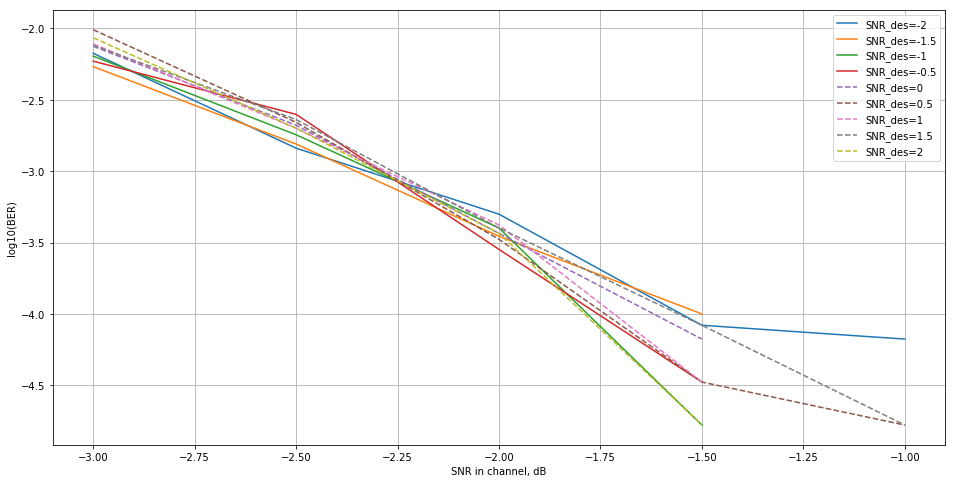
\includegraphics[width =0.6 \linewidth]{BAT_0_25}}
\caption{ метод: пар. Бх. Скорость 0.25}
\end{figure}
\begin{figure}[!h]
\center{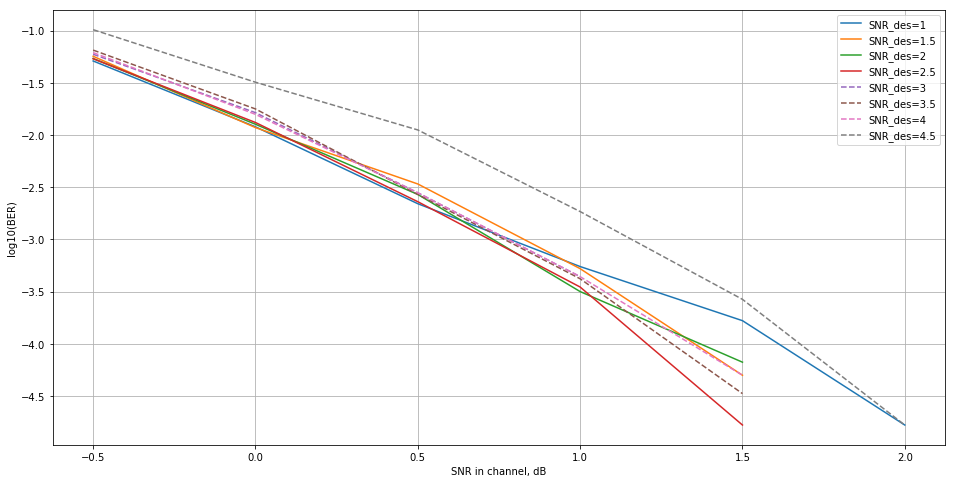
\includegraphics[width=0.6\linewidth]{BAT_0_5}}
\caption{ метод: пар. Бх. Скорость 0.5}
\end{figure}
\begin{figure}[!h]
\center{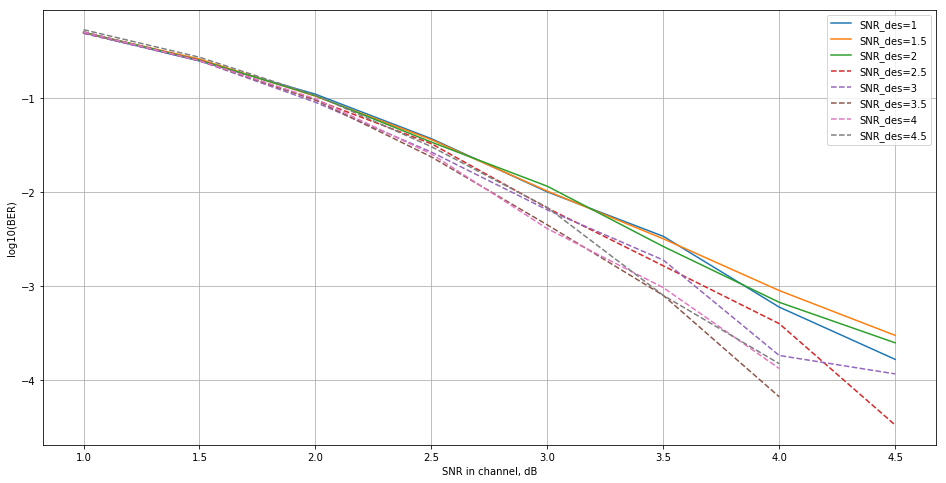
\includegraphics[width=0.6\linewidth]{BAT_0_75}}
\caption{метод: пар. Бх. Скорость 0.75}
\label{ris:image}
\end{figure}
Для исследования метода на основе оценки параметров Бхаттачариa были рассмотрены кодовые слова с длиной $ N = 512$ на трех скоростях: $R = 0.25$ (рис.2), $R = 0.5$ (рис.3) , $R = 0.75$ (рис.4). 


Исследуя полученные зависимости, можно сделать выводы:
\\
1) $R=0.25$: Самая эффективная оптимизация кода на $ SNR_{opt} =-1$
\\
2) $R=0.5$:  Самая эффективная оптимизация кода на $ SNR_ {opt} = 2.5$
\\
3) $R=0.75$: Самая эффективная оптимизация кода на $ SNR_{opt} = 3.5$


\\

Для метода на основе оценки вероятности ошибки аналогично были рассмотрены кодовые слова с длиной $n = 512$ на трех скоростях: $R =  0.25$ (рис.5), $R = 0.5$ (рис.6) , $R = 0.75$ (рис.7).
\\
\begin{figure}[!h]
\center{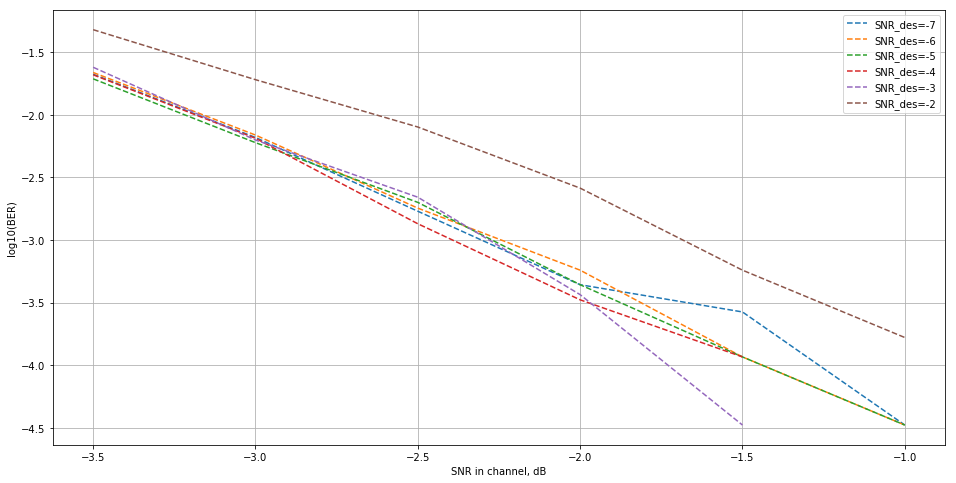
\includegraphics[width=0.6\linewidth]{DE_0_25}}
\caption{метод: эв. плот. Скорость 0.25. }
\end{figure}
\begin{figure}[!h]
\center{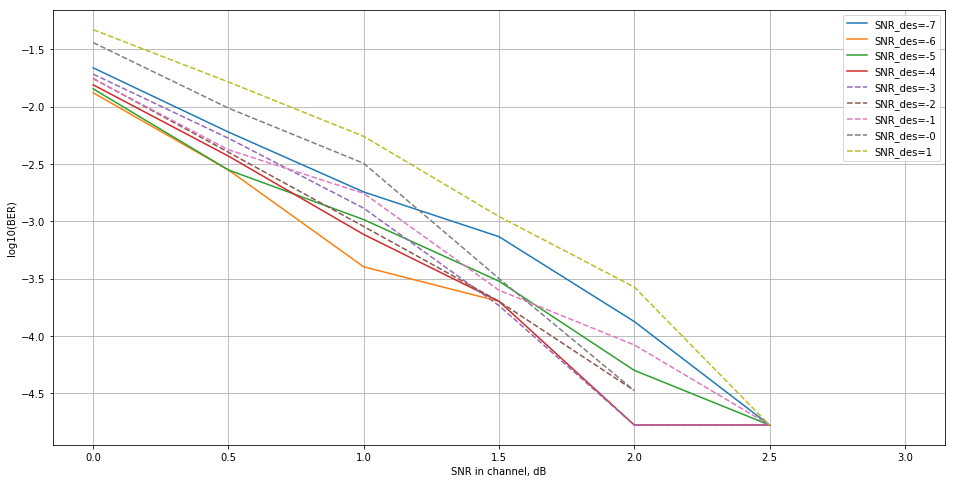
\includegraphics[width=0.6\linewidth]{DE_0_5}}
\caption{метод: эв. плот. Скорость 0.5.}
\end{figure}
\begin{figure}[!h]
\center{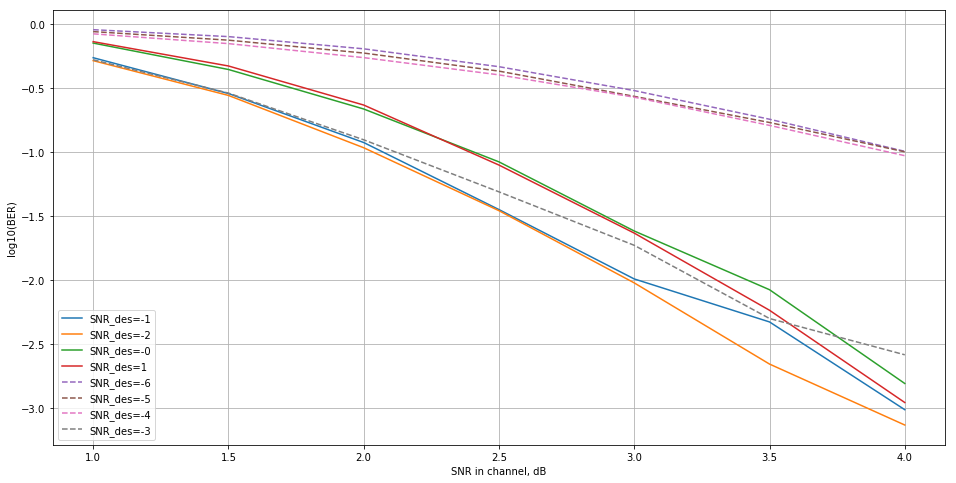
\includegraphics[width=0.6\linewidth]{DE_0_75}}
\caption{метод: эв. плот. Скорость 0.75.}
\label{ris:image}
\end{figure}
Здесь также видно, что есть определенные значения  параметра  $SNR_{opt}$, при которых код показывает наиболее высокую эффективность:
\\
1) $R=0.25$: Самая эффективная оптимизация кода на $ SNR_{opt} = -3$
\\
2) $R=0.5$:  Самая эффективная оптимизация кода на $ SNR_ {opt} = -6$
\\
3) $R=0.75$: Самая эффективная оптимизация кода на $ SNR_{opt} = -2$


\newpage
Сравним два метода при оптимальных параметрах:
\begin{figure}[!h]
\center{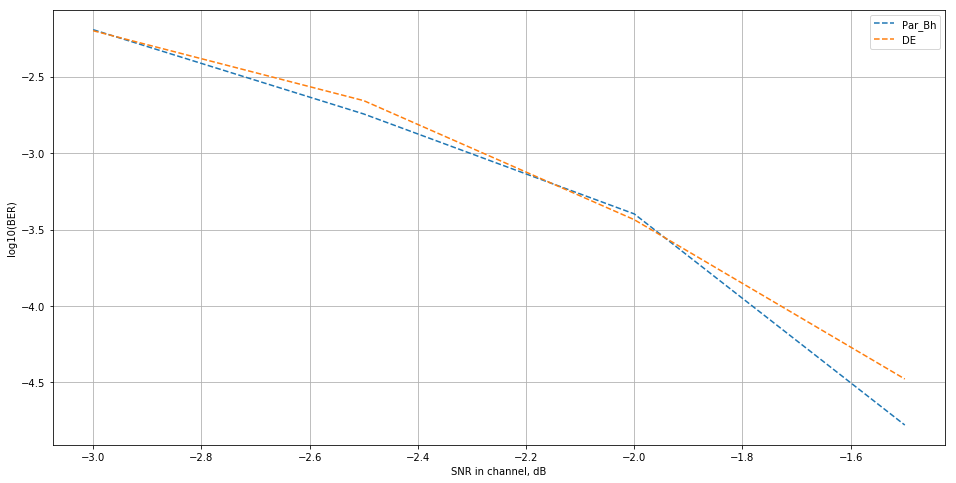
\includegraphics[width=0.6\linewidth]{com_0_25}}
\caption{Сравнение на опт. параметрах. Скорость 0.25.}
\label{ris:image}
\end{figure}
\begin{figure}[!h]
\center{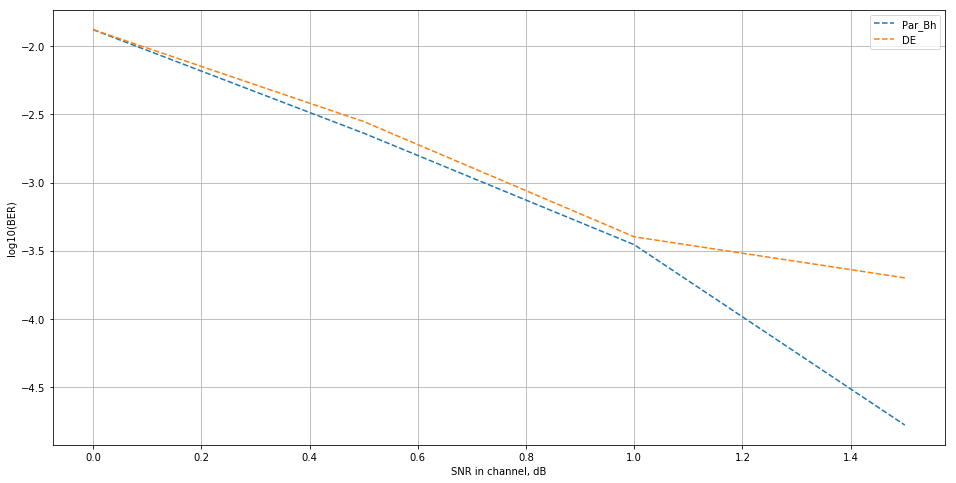
\includegraphics[width=0.6\linewidth]{com_0_5}}
\caption{Сравнение на опт. параметрах. Скорость 0.5.}
\label{ris:image}
\end{figure}
\begin{figure}[!h]
\center{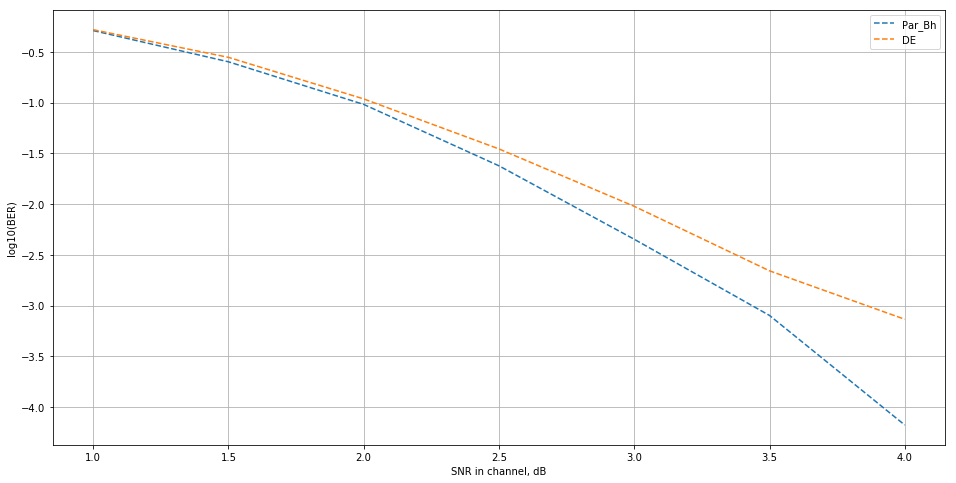
\includegraphics[width=0.6\linewidth]{com_0_75}}
\caption{Сравнение на опт. параметрах. Скорость 0.75.}
\label{ris:image}
\end{figure}
\newpage


\section{Заключение}

В результате моделирования показано, что метод на основе верхней оценки параметров Бхаттачариa, показывает большую эффективность, чем метод с оценкой вероятности ошибки (DE) на рассмотренных скоростях. Кроме того, за счет поиска оптимальных параметров построения кода, удалось добиться значительного увеличения эффективности кода. 
%Тут необходимо подытожить работу, еще раз написать, что именно было сделано и указать самые интересные закономерности (н-р в такой то области лучше этот метод, а в такой то этот)



\section*{Благодарности}
Исследование выполнено в ИППИ РАН при финансовой поддержке РНФ в рамках научного проекта No 14-50-00150.

\begin{thebibliography}{99}
%DONE
\bibitem{Arikan} {E. Arıkan.:} Channel Polarization: A Method for Constructing
Capacity-Achieving Codes for Symmetric
Binary-Input Memoryless Channels. IEEE
Trans. Inf. Theory, vol. 55, no. 7, pp. 3051–3073, Jul. 2009.
\bibitem{Trifonov} {P. Trifonov.:} Efficient Design and Decoding of Polar Codes. IEEE
Trans. Inf. Theory, vol.60, no. 11, pp.3221-3227, Nov. 2012.
\bibitem{Pfister}{H. D. Pfister.:} A Brief Introduction to Polar Codes. Supplemental Material for Advanced Channel Coding
\bibitem{TalVardy}{I.Tal, A. Vardy.:} List Decoding of Polar Codes.  IEEE
Trans. Inf. Theory, vol.1, no. 5, pp. 2213-2226, May. 2015.
\bibitem{MoriTanaka}{R.Mori.,T.Tanaka:} Performance of Polar Codes with the Construction using Density Evolution. IEEE Communication Letters, vol. 13, no. 7,pp. 519 -521, Jul. 2009.

\end{thebibliography}


\end{document}
